%1-光纤传感器

%文档类型
\documentclass[a4paper]{article}%A4纸,文档类型为论文

%宏包
%文字设置
\usepackage[UTF8]{ctex}%处理中文
\usepackage{xeCJK}%处理中文
\usepackage{fontspec,xunicode,xltxtra}%字体设置
%文档&排版设置
\usepackage{titlesec}%自定义章节标题样式
\usepackage{multicol}%分栏
\usepackage{hyperref}%超链接设置\daleth 
\usepackage{multirow,makecell}%制作复杂表格
\usepackage{booktabs}%画三线表要用
\usepackage{float}%图片、表格等位置浮动排版
\usepackage{indentfirst}%首行缩进
\usepackage{graphicx,subfigure}%图片插入
\usepackage{listings}%代码高亮
\usepackage{xcolor}
\usepackage{appendix}%附录
\usepackage{fancyhdr}%页眉页脚
\usepackage{geometry}%页边距
\usepackage{caption}
%数学
\usepackage{amsmath,amssymb}%公式
\usepackage{amsfonts,mathrsfs,txfonts}%数学字体
\usepackage{array}%矩阵
\usepackage{gensymb}%角度单位“度”的命令:\degree

\geometry{a4paper,scale=0.8}%设置了纸张为a4,并且版心占页面长度的比例为80%;scale也可以改为ratio,表示版面边距占页面长度的比例.
\hypersetup{colorlinks=true,linkcolor=black,citecolor=black}%去掉目录等超链接所带的红框,并让参考文献的引用颜色为黑色
\setlength{\parindent}{2em}%首行缩进2字符
\lstset{
    columns=fixed,
    numbers=left, % 在左侧显示行号
    numberstyle=\footnotesize\color{darkgray},% 设定行号格式
    backgroundcolor=\color[RGB]{245,245,244},% 设定背景颜色
    keywordstyle=\color[RGB]{40,40,255},% 设定关键字颜色
    numberstyle=\color[RGB]{0,192,192},%行号数字样式
    commentstyle=\it\color[RGB]{0,96,96},% 设置代码注释的格式
    stringstyle=\rmfamily\slshape\color[RGB]{128,0,0},% 设置字符串格式
}
\pagestyle{fancy}%页眉页脚
\fancyhead{}%清空页眉
\fancyhead[C]{\emph{实验报告-光纤传感器}}


\newcommand{\kaiti}{\CJKfamily{STKaiti}} % 楷体:\kaiti或\emph
\newcommand{\fs}{\CJKfamily{STFangsong}} % 仿宋:\fs或\fangsong
%黑体:\heiti

\newcommand{\suo}{\indent}%缩进2个字符

\title{\heiti{实验报告}}%标题
\author{{\emph{李佩哲}}}
\date{\emph{\small\today}}

\begin{document}

\begin{center}
\center{\bf{\LARGE{实验报告}\\\large{光纤传感器}}}\\
\emph{李佩哲~~~PB21051049~~~\\\today}
\end{center}

\section{实验目的}
学习并理解掌握光纤传输光的基本原理与分类,透射型、反射型、微弯型光纤传感器的原理和工作特点.

\section{实验原理}
\subsection{透射式光纤位移传感}
透射式光纤位移传感是一种强度型光纤传感,强度调制光纤传感器的基本原理是待测物理量引起光纤中的传输光光强变化,通过检测光强的变化实现对待测量的测量,
实验通过改变两透射多模光纤 出光芯径的相对位置(横向或者纵向)观测传输功率的变化,从而绘制功率随横向或纵向位移的关系曲线.

\subsection{反射式光纤位移传感}
反射式光纤传感实验的光纤探头由两根光纤组成,一根用于发射光,一根用于接收反射回来的光,由发射光纤发出的光照射到反射材料上,通过检测反射光的强度变化,就能测出反射体的位移.


\subsection{微弯型光纤传感器}
当光纤发生弯曲时,由于其全反射条件被破坏,纤芯中传播的某些模式光束进入包层,造成光纤中的能量损耗.

\section{实验仪器}
透射式光纤,反射式光纤,微弯型光纤,激光光源,探测器

\section{测量记录}
原始数据见附件.\\整理如下
\begin{table}[H]
  \begin{minipage}{0.2\linewidth}
      \centering
      \begin{tabular}{cc}
          \toprule
          $z$~/~cm & $P$~/~$\mu$W\\
          \midrule
          0.00	&	61.00	\\
          0.05	&	58.80	\\
          0.10	&	54.75	\\
          0.15	&	50.55	\\
          0.20	&	45.15	\\
          0.25	&	38.45	\\
          0.30	&	32.65	\\
          0.35	&	28.55	\\
          0.40	&	27.30	\\
          0.45	&	24.45	\\
          0.50	&	22.00	\\
          0.55	&	19.50	\\
          0.60	&	17.45	\\
          0.65	&	15.35	\\
          0.70	&	13.55	\\
          0.75	&	11.70	\\
          0.80	&	10.35	\\
          0.85	&	9.050 	\\
          0.90	&	7.905 	\\
          0.95	&	6.925 	\\
          1.00	&	6.230 	\\
          1.05	&	5.650 	\\
          1.10	&	5.140 	\\
          1.15	&	4.680 	\\
          \bottomrule
      \end{tabular}
      \caption{透射式光纤位移传感(纵向)}\label{001}
  \end{minipage}
  \begin{minipage}{0.29\linewidth}  
      \centering
      \begin{tabular}{cc} 
          \toprule
          $r$~/~cm & $P$~/~$\mu$W \\
          \midrule
          -0.13 	&	0	\\
          -0.12 	&	0.000150 	\\
          -0.11 	&	0.000750 	\\
          -0.10 	&	0.007740 	\\
          -0.09 	&	0.3028 	\\
          -0.08 	&	1.295 	\\
          -0.07 	&	2.975 	\\
          -0.06 	&	5.350 	\\
          -0.05 	&	8.460 	\\
          -0.04 	&	18.350 	\\
          -0.03 	&	42.000 	\\
          -0.02 	&	61.300 	\\
          -0.01 	&	64.250 	\\
          0.00 	&	64.300 	\\
          0.01 	&	61.600 	\\
          0.02 	&	45.530 	\\
          0.03 	&	27.300 	\\
          0.04 	&	11.200 	\\
          0.05 	&	5.520 	\\
          0.06 	&	1.980 	\\
          0.07 	&	0.7205 	\\
          0.08 	&	0.06310 	\\
          0.09 	&	0.002300 	\\
          0.10 	&	0.002050 	\\
          0.11 	&	0.000025 	\\
          0.12 	&	0	\\
          \bottomrule
      \end{tabular}
      \caption{透射式光纤位移传感(横向)}\label{002}
  \end{minipage}
  \begin{minipage}{0.29\linewidth}
    \centering
    \begin{tabular}{cc}
        \toprule
        $z$~/~cm & $P$~/~nW\\
        \midrule
        0.00 	&	534.5 	\\
        0.05 	&	537.7 	\\
        0.10 	&	537.0 	\\
        0.15 	&	532.5 	\\
        0.20 	&	523.5 	\\
        0.25 	&	512.0 	\\
        0.30 	&	495.5 	\\
        0.35 	&	476.0 	\\
        0.40 	&	455.0 	\\
        0.45 	&	434.4 	\\
        0.50 	&	413.7 	\\
        0.55 	&	396.5 	\\
        0.60 	&	376.7 	\\
        0.65 	&	360.3 	\\
        0.70 	&	341.3 	\\
        0.75 	&	323.3 	\\
        0.80 	&	304.0 	\\
        0.85 	&	284.5 	\\
        0.90 	&	267.3 	\\
        0.95 	&	252.5 	\\
        1.00 	&	238.8 	\\
        1.05 	&	226.2 	\\
        1.10 	&	215.0 	\\
        1.15 	&	204.7 	\\
        1.20 	&	194.3 	\\
        1.25 	&	184.5 	\\
        1.30 	&	174.3 	\\
        1.35 	&	164.5 	\\
        1.40 	&	156.1 	\\
        1.45 	&	148.3 	\\
        1.50 	&	141.7 	\\
        \bottomrule
    \end{tabular}
    \caption{反射式光纤位移传感}\label{003}
\end{minipage}
\begin{minipage}{0.2\linewidth}
  \centering
  \begin{tabular}{cc}
    (续表)\\
      \toprule
      $z$~/~cm & $P$~/~nW\\
      \midrule
      1.55 	&	135.3 	\\
      1.60 	&	130.0 	\\
      1.65 	&	124.4 	\\
      1.70 	&	119.0 	\\
      1.75 	&	113.9 	\\
      1.80 	&	108.9 	\\
      1.85 	&	103.7 	\\
      1.90 	&	99.00 	\\
      1.95 	&	94.70 	\\
      2.00 	&	91.10 	\\
      2.05 	&	87.75 	\\
      2.10 	&	84.46 	\\
      2.15 	&	81.55 	\\
      2.20 	&	78.55 	\\
      2.25 	&	75.82 	\\
      2.30 	&	72.90 	\\
      2.35 	&	70.15 	\\
      2.40 	&	67.27 	\\
      2.45 	&	64.80 	\\
      2.50 	&	62.50 	\\
      2.55 	&	60.60 	\\
      2.60 	&	58.53 	\\
      2.65 	&	56.65 	\\
      2.70 	&	54.85 	\\
      2.75 	&	53.20 	\\
      2.80 	&	51.15 	\\
      2.85 	&	49.25 	\\
      2.90 	&	47.63 	\\
      2.95 	&	46.00 	\\
      3.00 	&	44.73 	\\
      \bottomrule
  \end{tabular}
  \caption*{反射式光纤位移传感(续表)}
\end{minipage}
\end{table}

\begin{table}[H]
\begin{minipage}{0.2\linewidth}
  \centering
  \begin{tabular}{cc}
      \toprule
      $\Delta x$~/~cm & $P$~/~$\mu$W\\
      \midrule
      0.00 	&	957.5 	\\
      0.05 	&	945.0 	\\
      0.10 	&	921.5 	\\
      0.15 	&	908.0 	\\
      0.20 	&	898.0 	\\
      0.25 	&	885.0 	\\
      0.30 	&	858.0 	\\
      0.35 	&	834.0 	\\
      0.40 	&	818.0 	\\
      0.45 	&	813.0 	\\
      0.50 	&	810.5 	\\
      0.55 	&	808.5 	\\
      0.60 	&	803.5 	\\
      0.65 	&	793.5 	\\
      0.70 	&	781.0 	\\
      0.75 	&	787.0 	\\
      0.80 	&	796.5 	\\
      0.85 	&	799.5 	\\
      0.90 	&	802.7 	\\
      0.95 	&	804.7 	\\
      1.00 	&	808.7 	\\
      \bottomrule
  \end{tabular}
\end{minipage}
\begin{minipage}{0.29\linewidth}
\centering
\begin{tabular}{cc}
  (续表)\\
    \toprule
    $\Delta x$~/~cm & $P$~/~$\mu$W\\
    \midrule
    1.05 	&	809.3 	\\
    1.10 	&	803.0 	\\
    1.15 	&	797.0 	\\
    1.20 	&	789.5 	\\
    1.25 	&	788.5 	\\
    1.30 	&	782.5 	\\
    1.35 	&	801.0 	\\
    1.40 	&	808.0 	\\
    1.45 	&	810.0 	\\
    1.50 	&	813.8 	\\
    1.55 	&	809.6 	\\
    1.60 	&	804.0 	\\
    1.65 	&	769.4 	\\
    1.70 	&	761.0 	\\
    1.75 	&	760.0 	\\
    1.80 	&	761.0 	\\
    1.85 	&	760.0 	\\
    1.90 	&	758.0 	\\
    1.95 	&	761.0 	\\
    2.00 	&	757.3 	\\
    \bottomrule
\end{tabular}
\end{minipage}
\begin{minipage}{0.29\linewidth}
  \centering
  \begin{tabular}{cc}
    (续表)\\
      \toprule
      $\Delta x$~/~cm & $P$~/~$\mu$W\\
      \midrule
      2.05 	&	763.0 	\\
      2.10 	&	787.0 	\\
      2.15 	&	783.5 	\\
      2.20 	&	772.0 	\\
      2.25 	&	778.7 	\\
      2.30 	&	779.3 	\\
      2.35 	&	774.5 	\\
      2.40 	&	785.0 	\\
      2.45 	&	789.7 	\\
      2.50 	&	792.0 	\\
      2.55 	&	792.4 	\\
      2.60 	&	792.8 	\\
      2.65 	&	792.5 	\\
      2.70 	&	788.5 	\\
      2.75 	&	781.0 	\\
      2.80 	&	777.7 	\\
      2.85 	&	775.0 	\\
      2.90 	&	770.0 	\\
      2.95 	&	765.7 	\\
      3.00 	&	761.0 	\\
      \bottomrule
  \end{tabular}
  \end{minipage}
  \begin{minipage}{0.2\linewidth}
    \centering
    \begin{tabular}{cc}
      (续表)\\
        \toprule
        $\Delta x$~/~cm & $P$~/~$\mu$W\\
        \midrule
        3.05 	&	757.7 	\\
        3.10 	&	755.5 	\\
        3.15 	&	753.8 	\\
        3.20 	&	750.0 	\\
        3.25 	&	746.0 	\\
        3.30 	&	741.4 	\\
        3.35 	&	735.5 	\\
        3.40 	&	731.3 	\\
        3.45 	&	729.7 	\\
        3.50 	&	726.8 	\\
        3.55 	&	722.0 	\\
        3.60 	&	717.2 	\\
        3.65 	&	710.0 	\\
        3.70 	&	702.7 	\\
        3.75 	&	697.5 	\\
        3.80 	&	692.2 	\\
        3.85 	&	688.1 	\\
        3.90 	&	684.7 	\\
        3.95 	&	682.2 	\\
        4.00 	&	681.0 	\\
        \bottomrule
    \end{tabular}
    \end{minipage}
    \caption{微弯型光纤传感器}\label{004}
\end{table}

\section{分析与讨论}
\subsection{透射式光纤位移传感}
对表\ref{001}、表\ref{002}中数据分别作图如下图\ref{00001}
\begin{figure}[H]%插入图片
  \centering%图片居中
  \subfigure[纵向位移$z$~/~cm]{%小图一的名称
      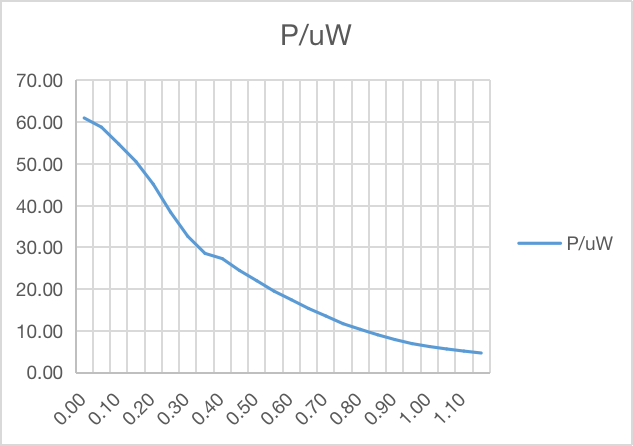
\includegraphics[scale=.525]{1.png}
      }
  \quad
  \subfigure[横向位移$r$~/~cm]{%小图二的名称
      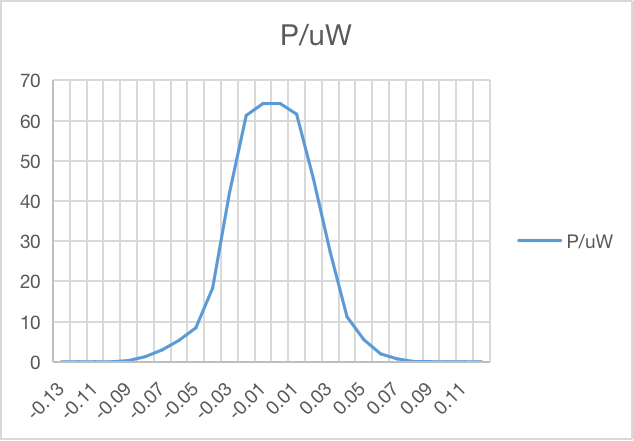
\includegraphics[scale=.525]{2.png}
      }
  \caption{功率$P$~/~$\mu$W~-~位移图}\label{00001}%总的图名称
\end{figure}
由图\ref{00001}可以看出,随着纵向位移$z$的增加,光功率逐渐减小,且随着$z$的增加减小速率逐渐降低;随着横向位移$r$的变化,光功率
在$r=0$处达最大值,且呈现关于$r=0$处的对称分布,随$\left| r \right|$的增加而减小,减小速率先变快后变慢.

\subsection{反射式光纤位移传感}
对表\ref{003}中数据作图如下图\ref{00002}
\begin{figure}[H]%插入图片
  \centering%图片居中
      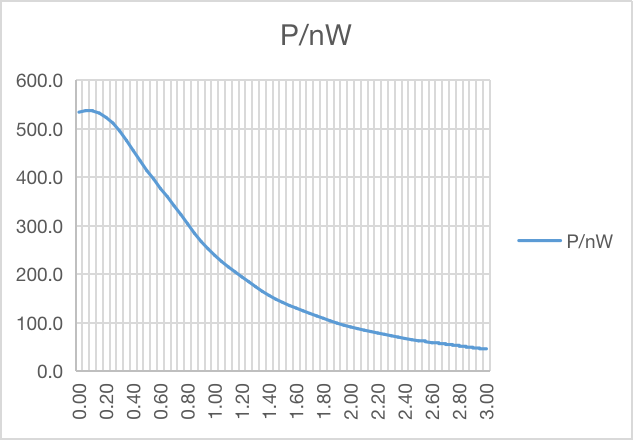
\includegraphics[scale=.7]{3.png}
  \caption{功率$P$~/~nW~-~纵向位移$z$~/~cm图}\label{00002}%总的图名称
\end{figure}
由图\ref{00002}可以看出,随着纵向位移$z$的增加,光功率先增加到一个峰值,后逐渐减小,减小速率随$z$的增加而变慢.

\subsection{微弯型光纤传感器}
对表\ref{004}中数据作图如下图\ref{00003}
\begin{figure}[H]%插入图片
  \centering%图片居中
      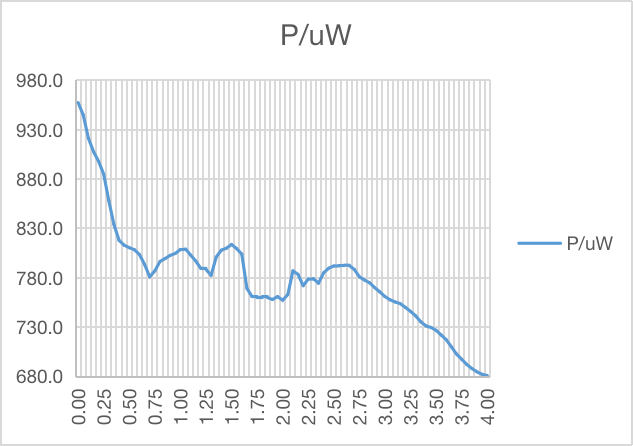
\includegraphics[scale=.7]{4.png}
  \caption{功率$P$~/~$\mu$W~-~变形程度$\Delta x$~/~cm图}\label{00003}%总的图名称
\end{figure}
由图\ref{00003}可以看出,随着变形程度$\Delta x$的增加,光功率总体上逐渐减小,且减小速率随$\Delta x$的增加而变快.

\section{总结与误差分析}
\subsection{总结}
通过本实验了解了光纤传输光全反射的基本原理,系统学习并掌握了投射式、反射式、微弯型光纤传感器的工作原理、使用方法与工作特点.\\
\suo 另外,反射式光纤的图像中光功率未从0开始变大,可能是由于调节纵向位移时未将光纤探头送到底所致;
微弯型光纤的图像出现较大问题,虽然总体呈下降趋势,但过程中出现了较大的起伏,且图像也未成理论上的抛物线,推测可能的问题有:实验时光源的出射光功率出现波动、
测量时光纤收到意料之外的挤压导致变形于光功率损耗、光纤两侧接口松动导致漏光等.

\subsection{误差分析}
实验误差除了人对螺旋测微器读数的随机误差外,还可能来自于仪器允差

\end{document}